\documentclass[main.tex]{subfiles}
\begin{document}
	\section{Lattices and crystal structure}
	\subsection{Theory} \label{sec:lattice_theory}
	There are three parts to the description of a crystal structure. First is the lattice. This is the mathematical "framework" upon which the physical part of the crystal lies. It can be defined in a number of ways, however the one we will use here is the following:
	
	\textbf{A lattice is defined as the infinite set of points produces by a linear combination of independent \emph{primitive lattice vectors}, with integer coefficients.}
	
	Usually, the primitive lattice vectors are labelled $ \V{a}_i $, and the coefficients $ n_i $, so for a $ d $-dimensional lattice, the lattice points $ \V{R} $ are given by
	\begin{equation}\label{eq:lattice_points}
	R = \sum_{i = 1}^{d} n_i \V{a}_i
	\end{equation}
	For this thesis we will mainly focus on the cases of $ d = 3 $ (visualization of lattices, families of lattice planes and scattering) and $ d = 2 $ (visualization of the Fermi surface).
	
	A thing to note, is that the choice of primitive lattice vectors is not unique. A new set of primitive lattice vectors can be created by taking a linear combination of the original primitive lattice vectors, with integer coefficients. If the original set is ordered in a matrix $ A = \begin{pmatrix*} \V{a}_1 & \V{a}_2 & \cdots & \V{a}_n \end{pmatrix*}$, and the new set in a matrix $ B = \begin{pmatrix*} \V{b}_1 & \V{b}_2 & \cdots & \V{b}_n \end{pmatrix*} $, then $ B = MA $, where $ M $ is the matrix containing the coefficients. This matrix must have integer entries, and its inverse likewise.
	
	The integer entries of the direct matrix makes sure that any lattice point generated with the new set of primitive lattice vectors will also have integer coefficients when expressed in the old set of primitive lattice vectors. The integer entries of the inverse matrix then makes sure that this process will also happen in reverse. This characteristic will come into play when trying to detect the lattice based on the users input of primitive lattice vectors.
	
	The second part is the unit cell. This is the building block of the lattice. It is a region of space which, when stacked will completely tile the space. Like with the choice of primitive lattice vectors, the choice of unit cell is not unique. In particular we distinguish between two type of unit cells: the smallest possible unit cell and everything else. The smallest possible unit cell is called a \textit{primitive} unit cell, and must contain only one lattice point (it cannot contain no lattice points, as then it would not recreate the lattice when tiled). Any unit cell containing more than one lattice point is called a \textit{conventional unit cell}. Usually a conventional unit cell is chosen for ease of calculation (as we will see in the scattering simulation), where the primitive lattice vectors constitute an orthogonal set.
	
	The third part of the crystal structure is the basis. This is a description of the physical objects that make up the structure, and their position in relation to the lattice. In our case the objects are of course atoms. 
	
	The basis is specified as a list of vectors that are to be added to the lattice points, specifying the position of the atoms in the crystal.
	
	The user can create any type of crystal they want by specifying any set of primitive lattice vector and supplying any desired basis. However a small selection of crystals will be available as presets. These include the 14 Bravais lattices with a 1 atom basis (at $ (0,0,0) $), named in table \ref{tab:bravais}. Each of these will specify the primitive lattice vectors for a corresponding primitive unit cell. Furthermore five other crystal presets will be available, named in table \ref{tab:presets}. Specifications of all of these presets are available in the appendix \ref{app:lattice}.
	\begin{table}[H]
		\centering
		\begin{tabular}{|l|l|}
			\hline
			Simple cubic & base centred cubic (bcc) \\
			\hline
			face centred cubic (fcc) & tetragonal \\
			\hline
			body centred tetragonal & orthorhombic \\
			\hline
			body centred orthorhombic & face centred orthorhombic \\
			\hline
			base centred orthorhombic & simple monoclinic \\
			\hline
			base centred monoclinic & hexaonal \\
			\hline
			triclinic & rhombohedral \\
			\hline
		\end{tabular}
		\caption{The 14 Bravais lattices}
		\label{tab:bravais}
	\end{table}
	\begin{table}[H]
		\centering
		\begin{tabular}{|l|l|}
			\hline
			fcc, conventional & bcc, conventional \\
			\hline
			zincblende & wurtzite \\
			\hline
			diamond (zincblende with 1 atom) & \\
			\hline
		\end{tabular}
		\caption{Other available crystal presets}
		\label{tab:presets}
	\end{table}
	
	\subsection{Implementation}	
	\begin{wrapfigure}{r}{2in}
		\begin{center}
			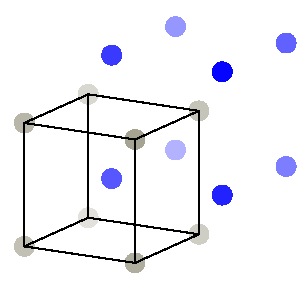
\includegraphics[width=\linewidth]{figures/lattice_unfinished_1.pdf}
		\end{center}
		\caption{One conventional unit cell for a bcc lattice. If we naively plot all atoms associated with a lattice point, we will end up with unfinished unit cells.}
		\label{fig:lattice_unfinished_1}
	\end{wrapfigure}
	Mathematically speaking, a lattice is infinite. A physical crystal, of course, is not. However, even though a real crystal is finite, plotting all of the atoms would be infeasible, both due to the number of atoms, each atom would be way too small (if it was feasible, what would be the point of this project then?). So for the purposes of this project, only a couple of unit cells will be plotted. A good amount seems to be 8 unit cells. 2 in each of the directions specified by the primitive lattice vectors. This keeps the size of the plot relatively small, whilst still showing the important parts of the crystal structure. As such, in the following we assume that $ n_i \in \{0, 1, 2\} $.
	
	In creating a program that plots these structures, the thought should always be on how the end product looks. Mainly we want the plot to be as clear and instructive as possible. This constitutes plotting only full unit cells: no unit cell can have missing atoms. However, the screen is still just a two dimensional projection of the actual three dimensional phenomena and without some form of depth perception, the crystal will just look like a weird two dimensional pattern. This is what grid lines fix. They give the required depth perception to allow the user to comprehend the crystal as a three dimensional structure, and not as a two dimensional sheet of dots. 
	
	For the crystals that can be expressed as a lattice with orthogonal primitive lattice vectors and a basis (cubic, tetragonal and orthorhombic), we usually want to plot orthogonal grid lines, whilst for other crystals plotting grid lines along the lattice vectors will be more useful.
	
	In the case of plotting primitive unit cells, the ones furthest away from the origin (say with $ n_1 = n_2 = n_3 = 2 $) may not be filled. Say the basis consists of only one atom. Then this atom will just be placed on the lattice points, and there is no problem, as this is the edge of the unit cell. However, if the basis consists of two atoms (or more), where one is placed at $ (0,0,0) $ and the other has some positive coordinates, then this second atom will be in a unit cell which is not supposed to be plotted (it would necessitate plotting the lattice points corresponding to $ n_i = 3 $). An example of this is figure \ref{fig:lattice_unfinished_1}, which shows one unit cell of a simple cubic lattice, with a two atom basis (corresponding to a conventional bcc unit cell). A way to correct for this is to write each plotted atom as a linear combination of the primitive lattice vectors with coefficients $ n'_i $ (where the coefficients here are real numbers, as they do not necessarily align with the lattice points). If the coefficients are $ 0 \leq n'_i \leq 2 $ for all $ n'_i $, then we plot the point.
	
	For plotting conventional unit cells when the user inputs primitive lattice vectors (for cubic, tetragonal and orthorhombic lattices), we need something similar, otherwise a situation like in figure \ref{fig:lattice_unfinished_2} may occur. To fix this we calculate the side lengths of the cuboid plot box that just contains the parallelepiped arising from plotting the lattice points with the specified coefficients ($ n_i \in \{0, 1, 2\}$), and fill this plot box completely with atoms.
	
	To calculate this, the program creates the 8 possible vectors arising from linear combinations of the primitive lattice vectors, with coefficients from the minimum and maximum coefficients and taking the limits of the plot box as the minimum and maximum values for these 8 vectors. For the specified lattice points, these 8 vectors are:
	\begin{equation}
		\begin{array}{llll}
			\V{v}_1 = \V{0}, & \V{v}_2 = 2\V{a}_1, & \V{v}_3 = 2\V{a}_2, & \V{v}_4 = 2\V{a}_3, \\
			\V{v}_5 = 2(\V{a}_1+\V{a}_2), & \V{v}_6 = 2(\V{a}_1+\V{a}_3), & \V{v}_7 = 2(\V{a}_2+\V{a}_3), &\V{v}_8 = 2(\V{a}_1+\V{a}_2+ \V{a}_3).
		\end{array}
	\end{equation}
	These are the vertices of the aforementioned parallelepiped. The side lengths of the plot box are then the maximum values of the coordinates minus the minimum values. Then we plot atoms for a larger range of coefficients to completely fill out this plot box. If some atoms fall outside of the box we hide them.
	
	\begin{wrapfigure}{r}{2in}
		\begin{center}
			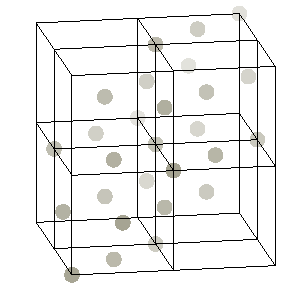
\includegraphics[width=\linewidth]{figures/lattice_unfinished_2.pdf}
		\end{center}
		\caption{An attempt to plot eight conventional unit cells for an FCC lattice, by using primitive lattice vectors with coefficients in the set $ \{0, 1, 2\} $. This does not fill out all eight unit cells, so we need to plot more lattice points than this. In practise we need $ \{-2, -1, 0, 1, 2, 3, 4\} $}
		\label{fig:lattice_unfinished_2}
	\end{wrapfigure}
	
	
	\subsection{Step-by-step}
	Initially the program will either load the chosen crystal preset in such a way as to make the resulting plot as informative as possible (eg. place lattice vectors along cardinal axes for an orthogonal lattice, to make plotting grid lines easier). If the user manually specifies the lattice and basis, the program will try to classify the lattice according to the specifications in the appendix \ref{app:lattice}. Next the program checks whether or not the crystal should be rotated to make plotting prettier.
	
	In general the rotation algorithm tries to align one lattice vector with the $ x $-axis. $ \V{a}_1 $ is preferred, but is only chosen to lie along the $ x $-axis if it forms an orthogonal pair with at least one other primitive lattice vector. The second primitive lattice vector of the pair ($\V{a}_2$ being preferred) is then aligned along the $ y $-axis. If the three primitive lattice vectors form an orthogonal set, then the last vector of the set will now be aligned along the $ z $-axis.
	
	The actual rotation is done by rotating the whole crystal (each primitive lattice vector and all vectors in the basis) along the cross product between the initial vector and the destination vector. Rotating the crystal such that $ \V{a}_1 $ lies along the $ x $-axis is done by rotating along $ \V{a}_1 \times \U{x} $, with an angle of $ \sin \theta = |\V{a}_1 \times \U{x}| / |\V{a}_1| $.
	
	However, this might rotate the crystal the wrong way, depending on the orientation between the two vectors. Because of this the program checks whether or not the rotated initial vector and the destination vector is parallel (that is, if the rotated $ \V{a}_1 $ is parallel to $ \U{x} $). If this is not the case, the whole crystal is rotated about the same vector, with an angle $ -2\theta $.
	
	Five of the Bravais lattices have specialised rotation functions: hexagonal, base centred monoclinic and the three face centred lattices.
	
	For the hexagonal, the program detects which primitive lattice vectors constitute the triangular lattice and orients them such that one is along the $ x $-axis and the other is in the $ xy $-plane (easily done by rotating the third primitive lattice vector such that it is parallel with the $ z $-axis). The same approach is used for the base centred monoclinic, but here the program always aligns $ \V{a}_1 $ along the $ x $-axis, and $ \V{a}_2 $ in the $ xy $-plane. Here however, the easy option of rotating $ \V{a}_3 $ is not available. Instead the program uses the fact that the vector rejection of $ \V{a}_2 $ with $ \V{a}_1 $ is orthogonal to $ \V{a}_1 $ (the vector rejection of $ \V{a}_2 $ with $ \V{a}_1 $ being $ \V{a}_2 $ minus the projection of $ \V{a}_2 $ along $ \V{a}_1 $). This vector rejection is then in the $ yz $-plane, and the crystal can be rotated along $ \V{a}_1 $ with the angle the rejection makes with $ \U{y} $: $ \cos \theta = \V{a}_{2,rej} \D \U{y} / |\V{a}_{2,rej}|$.
	
	For the face centred lattices, the ideal, rotated lattice is created from the magnitude of the primitive lattice vectors: if $ |\V{a}_1| = a, |\V{a}_2| = b, |\V{a}_3| = c $, then $ \V{a}'_1 = (a/2, b/2, 0), \V{a}'_2 = (a/2, 0, c/2), \V{a}'_3 = (0, b/2, c/2) $. First the crystal is rotated such that $ \V{a}_1 $ aligns with $ \V{a}'_1 $, by using their cross product. Then the crystal is rotated such that the now rotated $ \V{a}_2 $ aligns with $ \V{a}'_2 $, via the vector rejection of $ \V{a}_2 $ with $ \V{a}'_2 $. (\textbf{THIS METHOD AND THE ONE FOR THE HEXAGONAL LATTICE ASSUMES THAT THE PRIMITIVE LATTICE VECTORS ARE SPECIFIED AS IN THE APPENDIX}).
	
	With the lattice and basis rotated, the program finds the limits of the plot box as written above, after which the crystal is generated. This is done by looping over the three ranges specified by the minimum and maximum coefficients, creating each lattice point $ \V{R} $ by Eq. \eqref{eq:lattice_points}. For each lattice point $ n $ atomic positions are created by adding one of the $ n $ vectors in the basis to the lattice point. Furthermore lists of the colours and sizes associated with each atom are also created at this point. After creating all the atoms, the program deletes any that may lie outside the limits of the plot box.
	
	The only thing missing now is to create the grid lines and plot everything. The program has two ways of creating grid lines: along the primitive lattice vectors and along the cardinal axes.
	
	Creating grid lines along the primitive lattice vectors works by taking each lattice point $ \V{R}_n $, and finding the lattice point $ \V{R}_m $ the furthest away from it, in the (postive) direction of these lattice vectors, such that $ \V{R}_m = R_n + \alpha \V{a}_i $, where $ \alpha > 0 $, for all $ i \in [1,2,3] $, and creating lines between $ \V{R}_n $ and $ \V{R}_m $. This does create duplicate grid lines, but these do not show on the final plot, since they are all plotted with the same width and colour.
	
	Creating grid lines along the cardinal axes works by finding the minimum spacing between lattice points on these axes (called $ a_x, a_y$ and $ a_z $), and using these as the spacing between grid lines. The program then finds the maximum and minimum coordinates of lattice points along the cardinal axes (called $x_{min}, x_{max}$, etc.). This is used to create ranges corresponding to each lattice points on the cardinal axes: The range for the $ x $-axis starting at $ x_{min} $  and ending at $ x_{max} $ with steps of $ a_x $.
	
	These ranges then specify a grid of lattice points on the $ xy$, $ xz $ and $ yz $-planes. The program then creates lines orthogonal to these planes, stretching from $ z_{min} $ to $ z_{max} $ for the points in the $ xy $-plane, and similarly for the other two planes.
	
	Next a blank figure is created with an orthogonal projection and limits as calculated above. The atoms are plotted with colours and sizes specified by the user. The grid lines are plotted with a uniform size and colour and lastly the primitive lattice vectors are plotted with corresponding labels.
	
	\subsection{Examples}
	As an example, we plot a simple cubic lattice with a two atom basis (corresponding to the basis of a bcc lattice with conventional unit cells), where the atoms on the lattice points are grey and the body centred atoms are blue (figure \ref{fig:lattice_demo_1}), we write the following:
\begin{lstlisting}
Lattice(lattice_name="conventional bcc",
		colors=["xkcd:cement", "b"])
\end{lstlisting}
	Or we could plot a hexagonal lattice with a one atom basis (figure \ref{fig:lattice_demo_2}):
\begin{lstlisting}
Lattice(lattice_name="hexagonal")
\end{lstlisting}


	\begin{figure}[h]
		\centering
		\begin{minipage}{.4\textwidth}
			\centering
			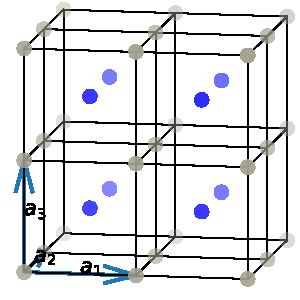
\includegraphics[width=2in]{figures/lattice_demo_1.pdf}
			\captionof{figure}{A simple cubic lattice with a two atom basis: One atom on the lattice points and another in the middle of each unit cell.}
			\label{fig:lattice_demo_1}
		\end{minipage}%
		\hfil
		\begin{minipage}{.4\textwidth}
			\centering
			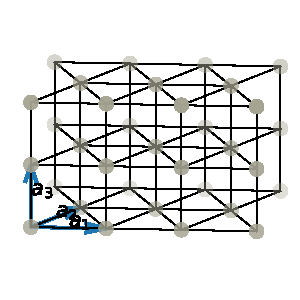
\includegraphics[width=2in]{figures/lattice_demo_2.pdf}
			\captionof{figure}{A hexagonal lattice, which consists of a series of triangular lattices stacked on top of each other.}
			\label{fig:lattice_demo_2}
		\end{minipage}
	\end{figure}
	
\end{document}